% Figure M9-Tabula-Muris hero: FACET on mouse Tabula Muris FACS tissues
% (Marrow + Spleen + Thymus) with native cell_ontology_class labels.
% Generated by experiments/m9_tabula_muris.py --hero.
\begin{figure}[t]
 \centering
 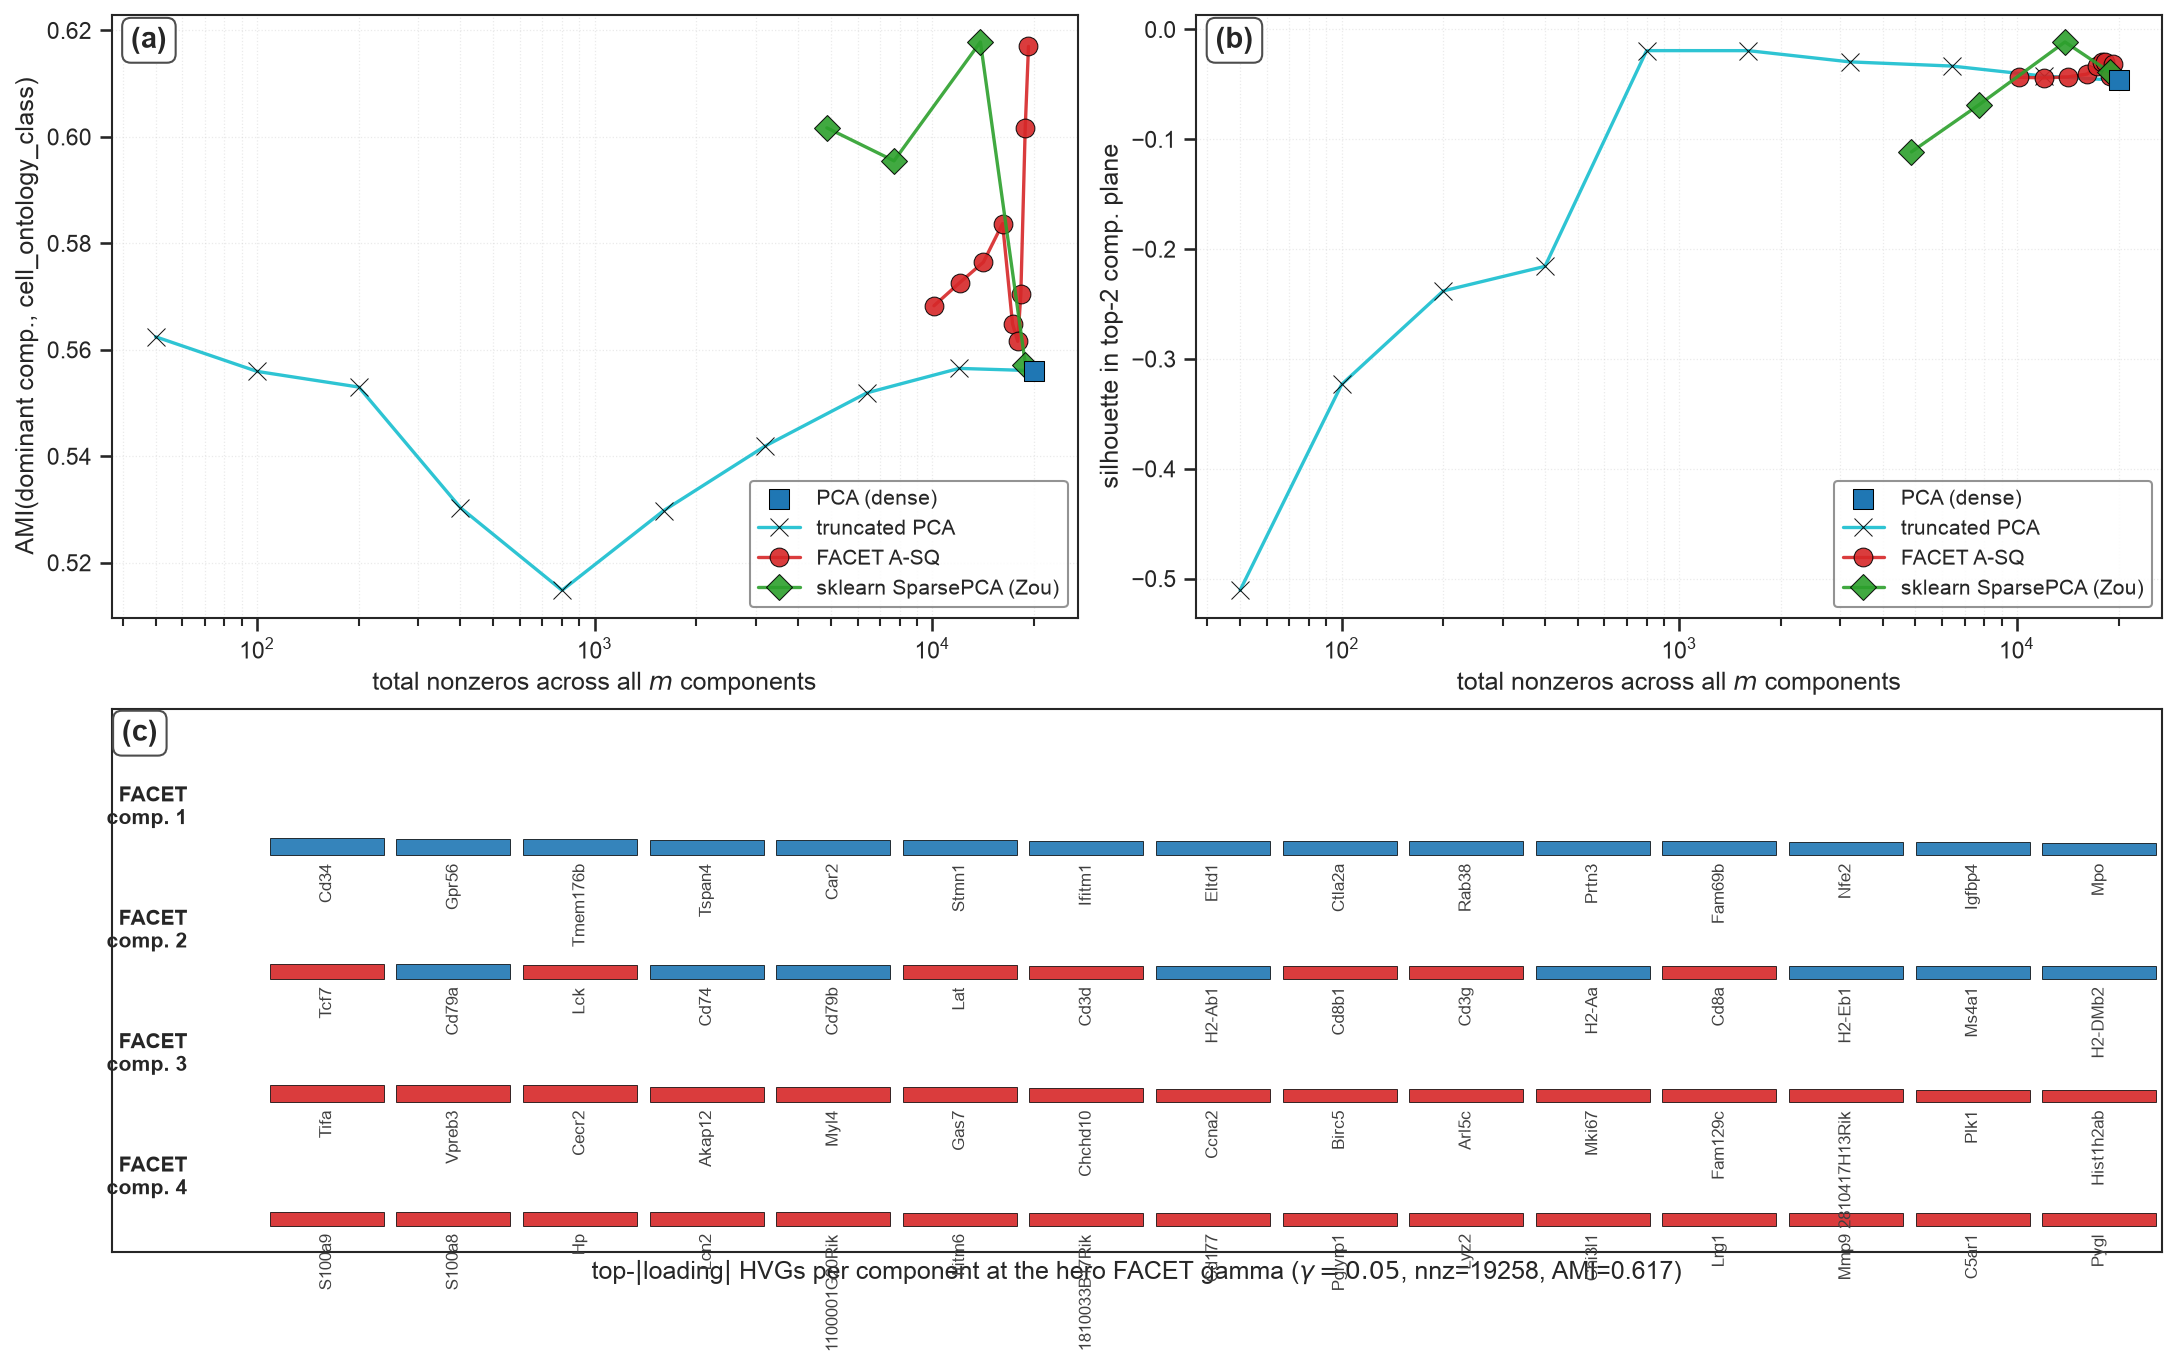
\includegraphics[width=\linewidth]{../shared/figures/generated/m9_tabula_muris_hero.png}
 \caption{\textbf{M9 Tabula Muris FACS (Marrow + Spleen + Thymus), native mouse cell-type labels.} 8{,}083 cells $\times$ 2{,}000 HVGs across $25$ \texttt{cell\_ontology\_class} categories; labels come from the official Tabula Muris annotations, not from any clustering of this matrix. $m{=}10$ components. \textbf{(a)}~AMI vs total nonzeros: FACET A-SQ reaches AMI $0.617$ against the dense-PCA ceiling of $0.556$ ($+0.061$, the largest margin of the three native-label scRNA experiments). \textbf{(b)}~Silhouette in the top-two component plane. \textbf{(c)}~Top-15 gene loadings per component at the hero FACET gamma; mouse symbols (title-case).}
 \label{fig:m9-tabula-muris-hero}
\end{figure}
